
\chapter{Requirements Specification}
%\setcounter{chapter}{2}
\renewcommand{\thechapter}{\Alph{chapter}}
\section{Introduction}

\subsection{Purpose}

The purpose of this document is to give a detailed description of the `Visualising Ant Colony Optimisation' application. This document will cover interface interactions and methods as well as providing definitions to important terminology. The document is primarily intended to be used as a reference point for the initial stages of development.

\subsection{Scope}

The `Visualising Ant Colony Optimisation' application is a desktop application which is designed to demonstrate the behaviour of an underlying ACO algorithms given various parameters. These parameters will be user defined and can be modified at their convenience. The algorithms behaviour given these parameters will be visible and the users can make a clear assessment about how each of the parameters impacts the algorithms performance.

During the background research into this subject area there does not seem to be too many applications which offer ACO visualisations and there are even less which provide a `friendly' environment which is simple and intuitive to use regardless of the users background knowledge.

The software will be deployed in an educational environment, with aims to provide a means for teaching ACO to students as part of an Artificial Intelligence course or for independent use as a self-learning exercise. As a result the software must cater for the majority of user groups to maximise its effectiveness. This means the software must be accessible on all major platforms and perform equally well on said platforms.

\subsection{Definitions}

\begin{table}[h]
\centering
\begin{tabular}{|l|l|lll}
\textbf{Term} & \textbf{Definition} \\ 
\hline
ACO & Ant Colony Optimisation \\ 
user & Anybody who is using or wishes to use the software \\ 
user group & A collective group of users representing different user needs. \\ 
interface &A graphical user interface \\
standalone &Operates independently of other hardware or software\\
agent &The entities which will be traversing the graph \\
\end{tabular}
\caption[Document Definitions]{Definitions for the keys terms used throughout this document}
\end{table}

\section{Overview}

This section will give an overview of the proposed application. This section will also expand on the expected user groups and functionality required by said groups. The constraints and assumptions will also be stated.

\subsection{Product Descriptive}

The software will be a standalone application that does not need to communicate with another system or application because of this, there is no need for any form of network connection to be present in order to use the application to its maximum potential.

The application will communicate with the Operating System on the host machine in order to enable the save and load functionalities through simple file input and output. However the user’s access to the host machines file system will be restricted by the fact that the saving and loading will be restricted to the user’s home directory preventing the overwriting of important documents.

The application itself will not take up too many system resources even if a large problem is being handled. This allows the users on a system or network to run the application without it impacting the performance of other services. Given that the target audience is educational establishments this is especially important as many teaching fellows have multiple applications running during a lesson or lecture and a negative impact on their system could reduce the amount of information taught during said session.

\subsection{Product functionality}

The users will be able to view a world which represents the Agents and the nodes. The state of this world will be directly related to the algorithm parameters specified by the users using the interface provided. There are several parameters which can be modified by the user, each of which will have a different impact of the state of the word and the algorithms behaviour.

The parameters which can be modified will be clearly labelled and will be clearly defined as editable. As these parameters will be user defined there will be strict error checking measures in place to catch any illegal values before they can cause problems for the algorithm in addition, each parameter will have a range of legal limits applied. This will prevent the users from entering values of the incorrect type (String when the systems needs a double) and will also prevent values from outside of the specified range being accepted. When a complication or error arises there will be a simple error message presented to the user informing them of both the error and why it occurred which should enable the user to resolve what they did incorrectly.

\subsection{User Groups and Characteristics}
\label{ssec:usergroups}
There will be three main user groups associated with this application. Each of these user groups will interact with the application in a slightly different manner but the main purpose and result will remain the same.

\noindent \\
\textbf{Teachers/Teaching fellows} will use the application with the underlying knowledge already in hand. They will be mainly be using the applications to visually portray ideas and will have expectations in regards to what to expect for a solution and will have some idea how the parameters impact the final result.

\noindent \\
\textbf{Students} will use the application with some background knowledge of the underlying concepts but will still use the application in an experimental manner and may have little expectations or understanding of how changing certain parameters impacts the final result. 

\noindent \\
\textbf{People new to the subject area} will use the application with potentially no idea about the underlying concepts. There will be measures in place to explain the underlying metrics and give an insight into what the application is actually doing. Given that they have less knowledge of this subject area that the other two user groups mentioned above, they will still be able to achieve the same results and levels of functionality. The application will cater for all users regardless of prior knowledge.

\begin{figure}[H]
\centering
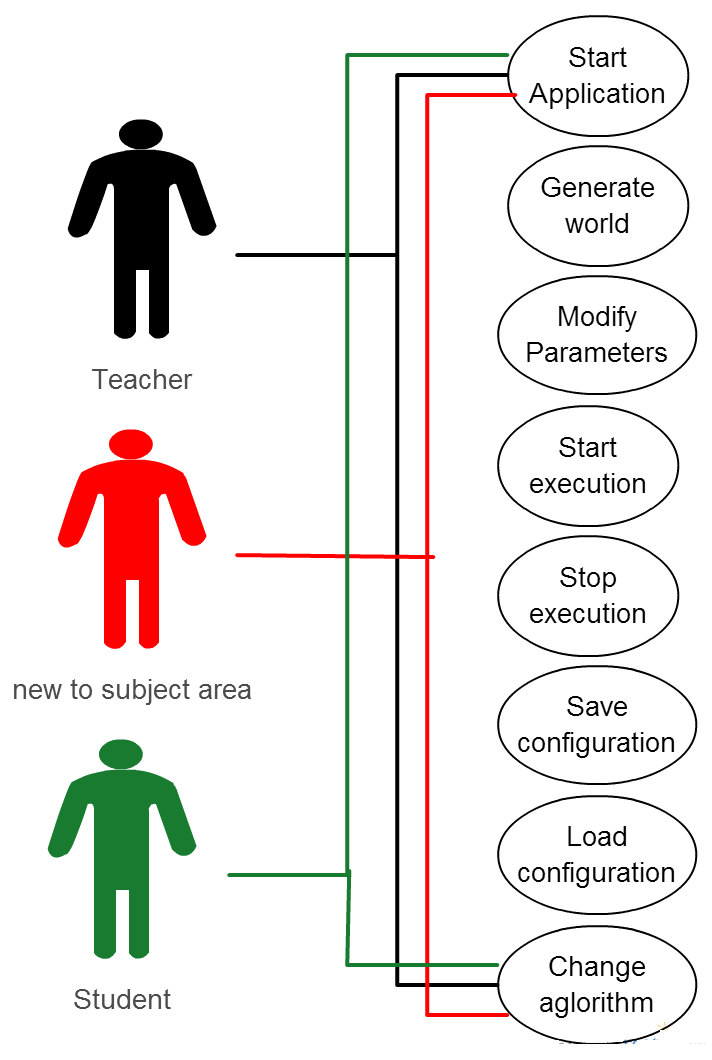
\includegraphics[scale=0.4]{Images/requirements/useCase}
\caption[Use Case Diagram]{Use Case Diagram showing how each of the above user groups can interact with the system. Regardless of the user, they can perform every action.}
\label{fig:useCase}
\end{figure}

\subsection{Constraints}

As the application is standalone is reduces the number of constraints which it becomes subject to. The main constraint which the application is associated with is the dimensions of the users display. The interface has to contain numerous elements in order to produce a simple and effective environment, thus it takes up quite a lot of screen real estate. However in modern times the amount of space required for the application to perform as expected is far from unreasonable and the application will be developed with this in mind.

The algorithm’s execution time is directly proportional to the user defined parameters, more specifically the number of agents and the number of nodes in the graph. The more agents and nodes the larger the execution time and resource requirements will be. The application will be developed with this in mind as there will be a constraint on how much memory and system resources the application should use. There is no expectation on the user to have a superfast high end machine therefore the application will be designed to accommodate a standard machine for these modern times.

The application does write the host systems file store so there must be adequate room to do so, however the files that will be written are simple text files which will not take up a lot of room on the host machines disk. Depending on the user’s machine this could still be a constraint. The responsibility and handling for this will belong to the user’s machine.

\subsection{Assumptions}

It will be assumed that the user will have the correct drivers installed and their machine will be able to handle the algorithms execution. The applications algorithms are not too resource intensive, therefore this is a reasonable assumption given the modern era and the advancement of computer technology.

It will be assumed that users will meet the minimum display requirements thus no dynamic resizing of the interface based on the users display dimensions will be performed. This significantly reduces complexity.

Another assumption is that every user will have some experience of using similar software and the interface will be familiar and therefore will be easy to use and navigate. The interface will use traditional methods such as simple buttons, text boxes and drop down menus to provide the user access to certain functionality.

\section{Specific Requirements}

This section contains the function requirements of the software as well as giving details about the different interfaces.

\subsection{User Interface}

There will be one main user interface for this application. This interface will contain a display area which is where the algorithms current state of execution will be represented visually to the user. There will also be an area which will house the text boxes which will be used by the user to interact with the algorithm and modify the parameters.

The display area will be simple and will be clearly identifiable. The text boxes responsible for handling user inputs will be clearly labelled so the user knows exactly what parameter they will be modifying. The text boxes will be obviously editable and the user will associate the look and feel of these text boxes with the fact that their contents can be modified.

The display will represent everything about the algorithms current state. This will display all of the graphs Nodes and all of the Agents at their current Node. The display area will also show the current pheromone levels for each connecting edge for a given node, this will be done in a way that is clear and understandable by all of the user groups identified in section \ref{ssec:usergroups}.

There will also be a textual representation of the current best agent. This will display the best route and the distance of the best route and will update as the global best is updated. There will also be textual representations of how many agents are currently working in addition to how many agents have finished.

\subsection{Hardware Interface}

The application does not require any specific hardware or host environment as it will be fully cross-platform compliant there are no direct hardware interfaces. There is no network use in this application thus there is no need to communicate with network adapters or anything of similar nature. The system interactions between this application and the host's Operating System file system will be delegated to the Operating System itself.

\subsection{Functional Requirements}
\label{funcreq}
\textbf{ID: FR1}\\
Title: Launch the Application\\
Description: Regardless of the users host environment the application should be able to be launched by the user using an executable .jar file.\\
Dependencies: None
\\

\noindent
\textbf{ID: FR2}\\
Title: Generate a World\\
Description: The user must be able to randomly generate a world for the algorithm to be executed on.\\
Dependencies: FR1
\\

\noindent
\textbf{ID: FR3}\\
Title: Visualise a World\\
Description: The user must be able to visualise the world and its parameters including the number of agents, the agent locations and the number of nodes.\\
Dependencies: FR1, FR2
\\

\noindent
\textbf{ID: FR4}\\
Title: Provide a means to modify parameters\\
Description: The application must provide simple ways to modify the algorithms parameters.\\
Dependencies: FR1
\\

\noindent
\textbf{ID: FR5}\\
Title: Generate a World with specified values\\
Description: The user must be able to generate a world for the algorithm to be executed on. This world with have user defined properties such as the number of nodes and agents.\\
Dependencies: FR1, FR4, F10
\\

\noindent
\textbf{ID: FR6}\\
Title: Visualise the Pheromone\\
Description: Every edge in the graph will have its own pheromone value. This must be visually displayed to the user and correctly model the pheromone deposit and decay operations.\\
Dependencies: FR1, FR2, FR3, FR13
\\

\noindent
\textbf{ID: FR7}\\
Title: Visualise the Agents movement\\
Description: As the algorithm is executing the agents will move through the graph. The movement of these agents must be displayed to the user in a logical manner.\\
Dependencies: FR1, FR2, FR3, FR8
\\

\noindent
\textbf{ID: FR8}\\
Title: Start the Algorithm's execution\\
Description: There must be a simple way for the user to start the algorithms execution. \\
Dependencies: FR1
\\

\noindent
\textbf{ID: FR9}\\
Title: Stop the Algorithm's execution\\
Description: There must be a simple way for the user to stop the algorithms execution anytime the user wishes to. \\
Dependencies: FR1
\\

\noindent
\textbf{ID: FR10}\\
Title: Validate parameters\\
Description: As the users will be able to define their own parameter values there must be correct measures in place to ensure the values entered are legal. If they are indeed illegal then suitable error messages will be displayed. \\
Dependencies: FR1
\\

\noindent
\textbf{ID: FR11}\\
Title: Display the best path\\
Description: As the algorithm is performing its task there must be a way to display the current best result to the user. \\
Dependencies: FR1, FR2, FR3, FR5, FR7, FR8, FR12
\\

\noindent
\textbf{ID: FR12}\\
Title: Agents must be able to move between Nodes\\
Description: In order for algorithm to perform as expected there must be a way for each Agent to move between Nodes in the graph. \\
Dependencies: FR1, FR2, FR3
\\

\noindent
\textbf{ID: FR13}\\
Title: Model Pheromone operations\\
Description: There must exist a way for the algorithm to correctly deposit and decay pheromones on graph edges adhering to specific formulae. \\
Dependencies: FR1, FR2, FR3, FR11
\\

\noindent
\textbf{ID: FR14}\\
Title: Load Configuration from a file\\
Description: There must exist a way for the users to load a pre-existing configuration from a file of their choosing. This allows the algorithm to be executed on the same problem multiple times. \\
Dependencies: FR1, FR2, FR3
\\

\noindent
\textbf{ID: FR15}\\
Title: Save Configuration to a file\\
Description: There must exist a way for the users to save the current configuration to a file of their choosing. This allows the algorithm to be executed on the same problem multiple times. \\
Dependencies: FR1, FR2, FR3
\\

\noindent
\textbf{ID: FR16}\\
Title: Exit the application\\
Description: The user must be able to exit the application completely killing the process and freeing system resources. \\
Dependencies: FR1
\clearpage
\subsection{Requirement Evaluation}

Each of the functional requirements mentioned in section \ref{funcreq} differ in thier levels of importance. The dependencies field for each requirement donates which requirements must be completed before said requirement itself can be finished. As this is the case the following represents the order of importance for each functional requirement.

Each of the functional requirements mentioned in section \ref{funcreq} differ in importance levels. The dependencies field for each requirement donates which requirements must be completed before said requirement itself can be finished. As this is the case the following represents the order of importance for each functional requirement.

\begin{table}[h]
\centering
\begin{tabular}{|l|l|lll}
\textbf{Requirement} & \textbf{Dependant Requirements} \\ 
\hline
FR1 & , \begin{tabular}{@{}c@{}}FR2, FR3, FR4, FR5, FR6, FR7, FR8, FR9\\ FR10, FR11, FR12, FR13, FR14, FR15, FR16\end{tabular} \\ \hline
FR2 & FR3, FR6, FR7, FR11, FR12, FR13, FR14, FR15 \\ \hline
FR3 & FR6, FR7, FR11, FR12, FR13, FR14, FR15. \\ \hline
FR8 &FR7, FR11, FR13 \\ \hline
FR4 &FR5\\ \hline
FR5 &FR11\\ \hline
FR10 &FR5\\ \hline
FR12 &FR11\\ \hline
FR13 &FR6\\ \hline
FR7 &FR11\\ \hline
FR11 &\\ \hline
FR6 &\\ \hline
FR9 &\\ \hline
FR14 &\\ \hline
FR15 &\\ \hline
FR16 &\\ \hline
\end{tabular}
\caption[Functional Requirement Dependencies]{Table representing the Functional Requirements and which requirements are dependent on them.}
\label{frtable}
\end{table}

\noindent
As described in Table \ref{frtable} the number of dependant requirements a requirement has the more important it is to the progress of the application. FR1 is the first task that must be accomplished therefore every other requirement is dependent on this being completed. FR1 is the ability to launch the application, if the application cannot be launched then none of the other requirements can be completed, this is a critical requirement.

FR2 is another critical requirement which must be completed early in development as many other requirements are dependent on its completion. FR2 is the ability to generate a World. A World contains all the data that the algorithm needs in order to both execute and visualise, therefore if there is no way to generate a World there is no way to visualise or model the algorithms execution (FR3).

Apart from FR8 (start the algorithm’s execution) the remaining functional requirements are somewhat independent of each other and are less critical. However this does not mean that they can be avoided as they will be needed in the final application version.